Here is the math used in the process:\\
\\
The links below talks more about the quantification equations used in our math in the paper above. 
Alternately, the link to it is as follows:\\
\href{https://petapixel.com/2013/06/15/a-mathematical-look-at-focal-length-and-crop-factor/}{Link 1}\\
\href{https://www.scantips.com/lights/fieldofviewmath.html}{Link 2}
\\
\\
\begin{figure}[!hb]
   

   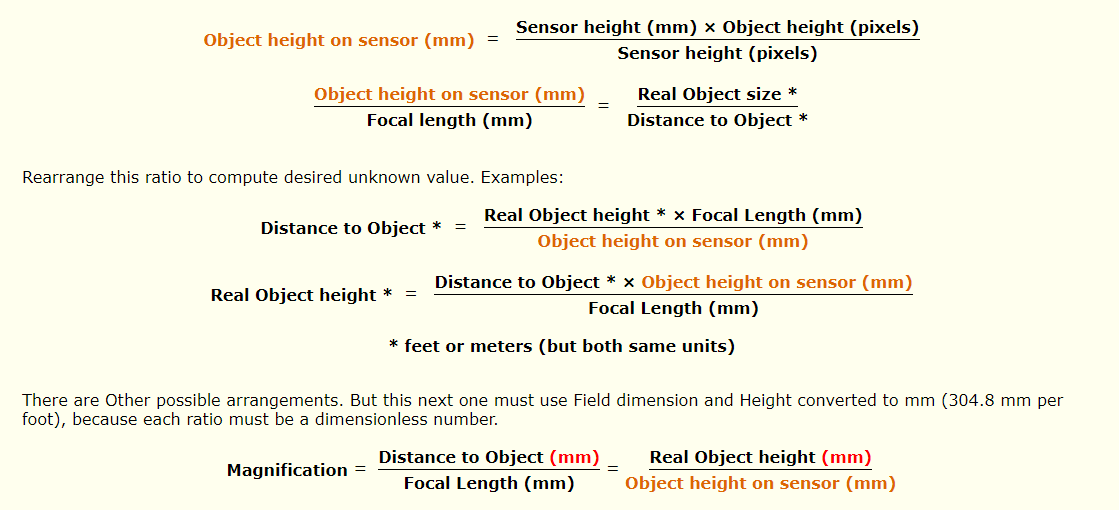
\includegraphics[scale=0.5]{images/MATH.PNG}

 
   \caption{Equations used in Quantification}\label{fig:GINIdataset}
\end{figure}
